%% -*- coding:utf-8 -*-
\chapter{Objects and morphisms}

\section{Equality}

The important question is how can we decide whenever an
object/morphism is equal to another object/morphism? The trivial
answer is possible for if an \mynameref{def:object} is a
\mynameref{def:set}. In this case we can say that 2 objects are equal
if they contains the same elements. Unfortunately we cannot do the
same for default objects as soon as they don't have any internal
structure. We can use the same trick as in
\mynameref{rem:set_vs_category}: if we cannot use ``microscope'' lets
use ``telescope'' and define the equality of objects and morphisms of
a category $\cat{C}$ in the terms of whole $\cathom{C}$.

\begin{definition}[Objects equality]
\label{def:object_equality}
Two \mynameref{def:object}s $a$ and $b$ in \mynameref{def:category}
$C$ are equal if there exists an unique \mynameref{def:isomorphism}
$f: a \to b$. This also means that also exist unique isomorphism $g: b
\to a$. These two \mynameref{def:morphism}s are related each other via
the following equations: $f \circ g = \idarrow[a]$ and $g \circ f
= \idarrow[b]$. 
\end{definition}

Unlike \mynameref{def:function}s between \mynameref{def:set}s we don't
have any additional info 
\footnote{
for instance info about sets internals. i.e. which elements of the sets
are connected by the considered functions
}
about \mynameref{def:morphism}s except
category theory axioms which the morphisms satisfied
\cite{bib:stackexchange:morphism:equality}. This leads us to the
following definition for morphims equality:
\begin{definition}[Morphisms equality]
\label{def:morphism_equality}
Two \mynameref{def:morphism}s $f$ and $g$ in \mynameref{def:category}
$C$ are equal if the equality can be derived from the base axioms: 
\begin{itemize}
\item \mynameref{axm:composition}
\item \mynameref{axm:associativity}
\item \mynameref{def:id}: \eqref{eq:leftid}, \eqref{eq:rightid}
\end{itemize}
or \mynameref{def:commutative_diagram}s which postulate the equality.
\end{definition}

As an example lets proof the following theorem
\begin{theorem}[Identity is unique]
\label{thm:identity_unique}
The \mynameref{def:id} is unique.
\begin{proof}
Consider an \mynameref{def:object} $a$ and it's \mynameref{def:id} 
$\idarrow[a]$. Let $\exists f: a \to a$ such that $f$ is also
identity. In the case \eqref{eq:leftid} for $f$ as identity gives
\[
f \circ \idarrow[a] = \idarrow[a].
\]
From other side \eqref{eq:rightid} for $\idarrow[a]$ satisfied
\[
f \circ \idarrow[a] = f
\]
i.e. $f = \idarrow[a]$.
\end{proof}
\end{theorem}

\section{Initial and terminal objects}
\begin{definition}[Initial object]
\label{def:initial_object}
Let $\cat{C}$ is a \mynameref{def:category}, the
\mynameref{def:object} $i \in \catob{C}$ is called
\textit{initial object} if $\forall x \in \catob{C}
\exists! f_x: i \to x \in \cathom{C}$.
\end{definition}

\begin{definition}[Terminal object]
\label{def:terminal_object}
Let $\cat{C}$ is a \mynameref{def:category}, the
\mynameref{def:object} $t \in \catob{C}$ is called
\textit{terminal object} if $\forall x \in \catob{C}
\exists! g_x: x \to t \in \cathom{C}$.
\end{definition}

As you can see the initial and terminal objects are opposite each
other. I.e. if $i$ is an \mynameref{def:initial_object} in $\cat{C}$
then it will be \mynameref{def:terminal_object} in
the \mynameref{def:op_category} $\cat{C^{op}}$.

\begin{theorem}[Initial object is unique]
\label{thm:initial_object_unique}
Let $\cat{C}$ is a category and $i, i' \in \catob{C}$ two
\mynameref{def:initial_object}s then there exists an unique
\mynameref{def:isomorphism} $u: i \to i'$ (see
\mynameref{def:object_equality}) 
\begin{proof}
Consider the following \mynameref{def:commutative_diagram} (see
\cref{fig:initial_object_unique}) 
\begin{figure}
  \centering
  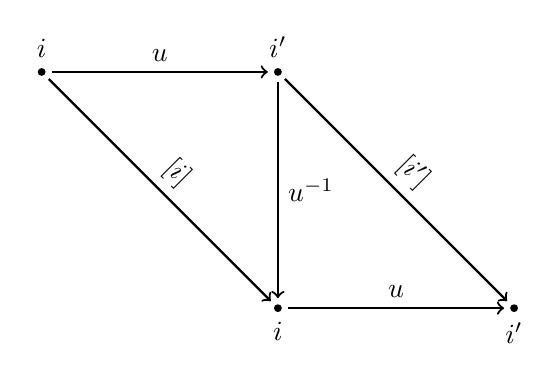
\begin{tikzpicture}[ele/.style={fill=black,circle,minimum
        width=.8pt,inner sep=1pt},every fit/.style={ellipse,draw,inner
        sep=-2pt}]

    % the texts
    
    \node[ele,label=above:$i$] (i1) at (0,3) {};    
    \node[ele,label=above:$i'$] (i2) at (3,3) {};    
    \node[ele,label=below:$i$] (i12) at (3,0) {};
    \node[ele,label=below:$i'$] (i22) at (6,0) {};

    \draw[->,thick,shorten <=2pt,shorten >=2pt] (i1) to
    node[sloped,above]{$u$} (i2);
    \draw[->,thick,shorten <=2pt,shorten >=2] (i12) to
    node[sloped,above]{$u$} (i22); 
    \draw[->,thick,shorten <=2pt,shorten >=2] (i1) to
    node[sloped,above]{$\idarrow[i]$} (i12); 
    \draw[->,thick,shorten <=2pt,shorten >=2] (i2) to
    node[sloped,above]{$\idarrow[i']$} (i22); 
    \draw[->,thick,shorten <=2pt,shorten >=2] (i2) to
    node[right]{$u^{-1}$} (i12); 
  \end{tikzpicture}
  \caption{Commutative diagram for initial object unique proof}
  \label{fig:initial_object_unique}
\end{figure}
\end{proof}
\end{theorem}

\begin{theorem}[Terminal object is unique]
\label{thm:terminal_object_unique}
Let $\cat{C}$ is a category and $t, t' \in \catob{C}$ two
\mynameref{def:terminal_object}s then there exists an unique
\mynameref{def:isomorphism} $v: t' \to t$ (see
\mynameref{def:object_equality}) 
\begin{proof}
Just got to the \mynameref{def:op_category} and revert arrows in
\cref{fig:initial_object_unique}. The result shown on
\cref{fig:terminal_object_unique} and it proofs the theorem statement.
\begin{figure}
  \centering
  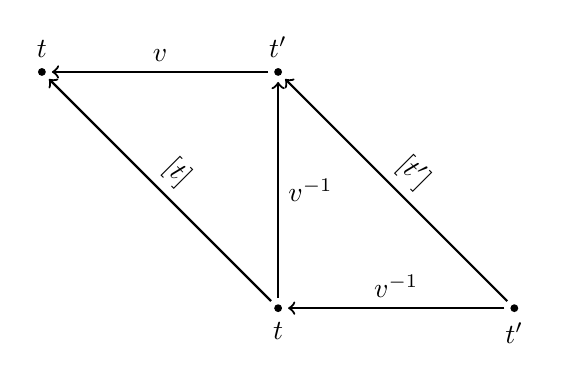
\begin{tikzpicture}[ele/.style={fill=black,circle,minimum
        width=.8pt,inner sep=1pt},every fit/.style={ellipse,draw,inner
        sep=-2pt}]

    % the texts
    
    \node[ele,label=above:$t$] (t1) at (0,3) {};    
    \node[ele,label=above:$t'$] (t2) at (3,3) {};    
    \node[ele,label=below:$t$] (t12) at (3,0) {};
    \node[ele,label=below:$t'$] (t22) at (6,0) {};

    \draw[->,thick,shorten <=2pt,shorten >=2pt] (t2) to
    node[sloped,above]{$v$} (t1);
    \draw[->,thick,shorten <=2pt,shorten >=2] (t22) to
    node[sloped,above]{$v^{-1}$} (t12); 
    \draw[->,thick,shorten <=2pt,shorten >=2] (t12) to
    node[sloped,above]{$\idarrow[t]$} (t1); 
    \draw[->,thick,shorten <=2pt,shorten >=2] (t22) to
    node[sloped,above]{$\idarrow[t']$} (t2); 
    \draw[->,thick,shorten <=2pt,shorten >=2] (t12) to
    node[right]{$v^{-1}$} (t2); 
  \end{tikzpicture}
  \caption{Commutative diagram for terminal object unique proof}
  \label{fig:terminal_object_unique}
\end{figure}
\end{proof}
\end{theorem}


\section{Product and sum}
The pair of 2 objects is defined via so called universal property in
the following way:
\begin{definition}
\label{def:product}
Let we have a category $\cat{C}$ and $c_1, c_2 \in \catob{C}$ -two
\mynameref{def:object}s the product of the objects $c_1, c_2$ is
another object in $\cat{C}$ $c = c_1 \times c_2$ with 2
\mynameref{def:morphism}s $\pi_1, \pi_2$ such that $a = g_a c, b = g_b
c$ and the 
following universal property is satisfied: $\forall c' \in \catob{C}$
and morphisms $\pi'_1: \pi'_2 c' = c_1, \pi'_2: \pi'_2 c' = c_2$, exists unique
morphism $h$ such that the following diagram (see \cref{fig:product})
commutes, i.e. $\pi'_1 = \pi_1 \circ h, \pi'_2 = \pi_2 \circ h$.
\begin{figure}
  \centering
  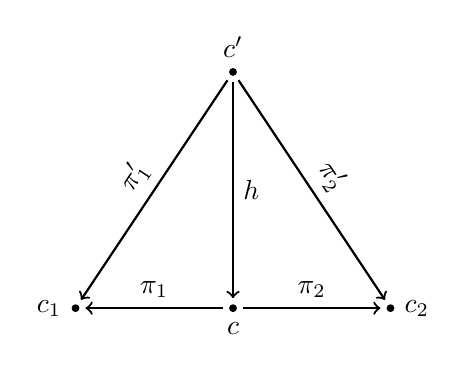
\begin{tikzpicture}[ele/.style={fill=black,circle,minimum
        width=.8pt,inner sep=1pt},every fit/.style={ellipse,draw,inner
        sep=-2pt}]

    % the texts
    
    \node[ele,label=left:$c_1$] (a) at (0,0) {};    
    \node[ele,label=right:$c_2$] (b) at (4,0) {};    
    \node[ele,label=below:$c$] (c) at (2,0) {};
    \node[ele,label=above:$c'$] (c') at (2,3) {};

    \draw[->,thick,shorten <=2pt,shorten >=2pt] (c) to
    node[sloped,above]{$\pi_1$} (a);
    \draw[->,thick,shorten <=2pt,shorten >=2] (c) to
    node[sloped,above]{$\pi_2$} (b); 
    \draw[->,thick,shorten <=2pt,shorten >=2] (c') to
    node[sloped,above]{$\pi'_1$} (a); 
    \draw[->,thick,shorten <=2pt,shorten >=2] (c') to
    node[sloped,above]{$\pi'_2$} (b); 
    \draw[->,thick,shorten <=2pt,shorten >=2] (c') to
    node[right]{$h$} (c); 
  \end{tikzpicture}
  \caption{Product $c = c_1 \times c_2$. $\forall c, \exists! h \in
    \cathom{C}: \pi'_1 = \pi_1 \circ h, \pi'_2 = \pi_2 \circ h$.}
  \label{fig:product}
\end{figure}
In other words $h$ factorizes $\pi'_{1,2}$.
\end{definition}

If we invert arrows in \mynameref{def:product} we will got another
object definition that is called sum

\begin{definition}
\label{def:sum}
Let we have a category $\cat{C}$ and $c_1, c_2 \in \catob{C}$ -two
\mynameref{def:object}s the sum of the objects $c_1, c_2$ is
another object in $\cat{C}$ $c = c_1 \oplus c_2$ with 2
\mynameref{def:morphism}s $i_1, i_2$ such that $c = i_1 c_1, c = i_2
c_2$ and the 
following universal property is satisfied: $\forall c' \in \catob{C}$
and morphisms $i'_1: i'_1 x_1 = c', i'_2: i'_2 x_2 = c'$, exists unique
morphism $h$ such that the following diagram (see \cref{fig:sum})
commutes, i.e. $i'_1 = h \circ i_1, i'_2 = h \circ i_2$.
\begin{figure}
  \centering
  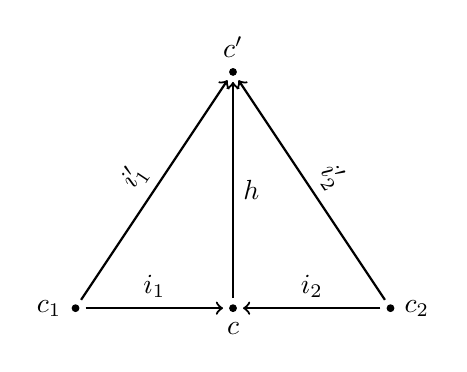
\begin{tikzpicture}[ele/.style={fill=black,circle,minimum
        width=.8pt,inner sep=1pt},every fit/.style={ellipse,draw,inner
        sep=-2pt}]

    % the texts
    
    \node[ele,label=left:$c_1$] (a) at (0,0) {};    
    \node[ele,label=right:$c_2$] (b) at (4,0) {};    
    \node[ele,label=below:$c$] (c) at (2,0) {};
    \node[ele,label=above:$c'$] (c') at (2,3) {};

    \draw[->,thick,shorten <=2pt,shorten >=2pt] (a) to
    node[sloped,above]{$i_1$} (c);
    \draw[->,thick,shorten <=2pt,shorten >=2] (b) to
    node[sloped,above]{$i_2$} (c); 
    \draw[->,thick,shorten <=2pt,shorten >=2] (a) to
    node[sloped,above]{$i'_1$} (c'); 
    \draw[->,thick,shorten <=2pt,shorten >=2] (b) to
    node[sloped,above]{$i'_2$} (c'); 
    \draw[->,thick,shorten <=2pt,shorten >=2] (c) to
    node[right]{$h$} (c'); 
  \end{tikzpicture}
  \caption{Sum $c = c_1 \oplus c_2$. $\forall c, \exists! h \in
    \cathom{C}: i'_1 = h \circ i_1, i'_2 = h \circ i_2 $.}
  \label{fig:sum}
\end{figure}
In other words $h$ factorizes $i'_{1,2}$.
\end{definition}

\section{Exponential}
TBD

\section{Programming languages and algebraic data types}
TBD

\section{Examples}

\subsection{\textbf{Set} category}
\begin{example}[Initial object][\textbf{Set}]
\label{ex:set_initial_object}
Note that there is only one function from empty set to any other sets
\cite{bib:proofwiki:Empty_Mapping_is_Unique} that makes the empty set
as the \mynameref{def:initial_object} in \mynameref{ex:setcategory}. 
\end{example}

\begin{example}[Terminal object][\textbf{Set}]
\label{ex:set_terminal_object}
\mynameref{def:terminal_object} in \mynameref{ex:setcategory} is a set
with one element i.e \mynameref{def:singleton_set}. 
\end{example}


\subsection{Programming languages}
In our toy example \cref{fig:pl_example} the type String is
\mynameref{def:initial_object} and type Bool is the
\mynameref{def:terminal_object}. From other side there are types in
different programming languages that satisfies the definitions of
initial and terminal objects.

\subsubsection{\textbf{Hask} category}
\begin{example}[Initial object][\textbf{Hask}]
If we avoid lazy evaluations in Haskell (see
\mynameref{rem:hask_lazy_eval}) then we can found the following types
as candidates for initial and terminal object in haskell. 
\label{ex:hask_initial_object}
\mynameref{def:initial_object} in \mynameref{ex:haskcategory} is a
type without values 
\begin{minted}{haskell}
data Empty
\end{minted}
i.e. you cannot construct a object of the type.

There is only one function from the initial object:
\begin{minted}{haskell}
absurd :: Empty -> a
\end{minted}
The function is called absurd because it does absurd action. Nobody
can proof that it does not exist. For the existence proof can be used
the following absurd argument: ``Just provide me an object type Empty
and I will provide you the result of evaluation''. 

There is no function in opposite direction because it would had been
used for the Empty object creation. 
\end{example}

\begin{example}[Terminal object][\textbf{Hask}]
\label{ex:hask_terminal_object}
Terminal object (unit) in \mynameref{ex:haskcategory} keeps only one element
\begin{minted}{haskell}
data () = ()
\end{minted}
i.e. you can create only one element of the type. You can use the
following function for the creation:
\begin{minted}{haskell}
unit :: a -> ()
unit _ = ()
\end{minted}
\end{example}

TBD
\subsubsection{\textbf{C++} category}
\begin{example}[Initial object][\textbf{C++}]
\label{ex:cpp_initial_object}
In C++ exists a special type that does not hold any values and as
result that cannot be created:
\begin{minted}{c++}
void
\end{minted}
You cannot create an object of that type: you will get a compiler
error if you try.
\end{example}

\begin{example}[Terminal object][\textbf{C++}]
\label{ex:cpp_terminal_object}
C++ 17 introduced a special type that keeps only one value: 
\begin{minted}{c++}
namespace std {
  struct monostate {};
}
\end{minted}
\end{example}


TBD
\subsubsection{\textbf{Scala} category}
\begin{example}[Initial object][\textbf{Scala}]
\label{ex:scala_initial_object}
We used a same trick as for \mynameref{ex:hask_initial_object} and define
\mynameref{def:initial_object} in \mynameref{ex:scalacategory} as a
type without values 
\begin{minted}{scala}
sealed trait Empty
\end{minted}
i.e. you cannot construct a object of the type.
\end{example}

\begin{example}[Terminal object][\textbf{Scala}]
\label{ex:scala_terminal_object}
We used a same trick as for \mynameref{ex:hask_terminal_object} and define
\mynameref{def:terminal_object} in \mynameref{ex:scalacategory} as a
type with only one value
\begin{minted}{scala}
abstract final class Unit extends AnyVal
\end{minted}
TBD
i.e. you can create only one element of the type.
\end{example}

TBD

\subsection{Quantum mechanics}
TBD

